
\documentclass[11pt]{article}
\usepackage{a4wide}
\usepackage[dvips]{graphicx}
\newcommand{\printindex}[0]{} %recover pod2latex bug
\begin{document}
\begin{center}
    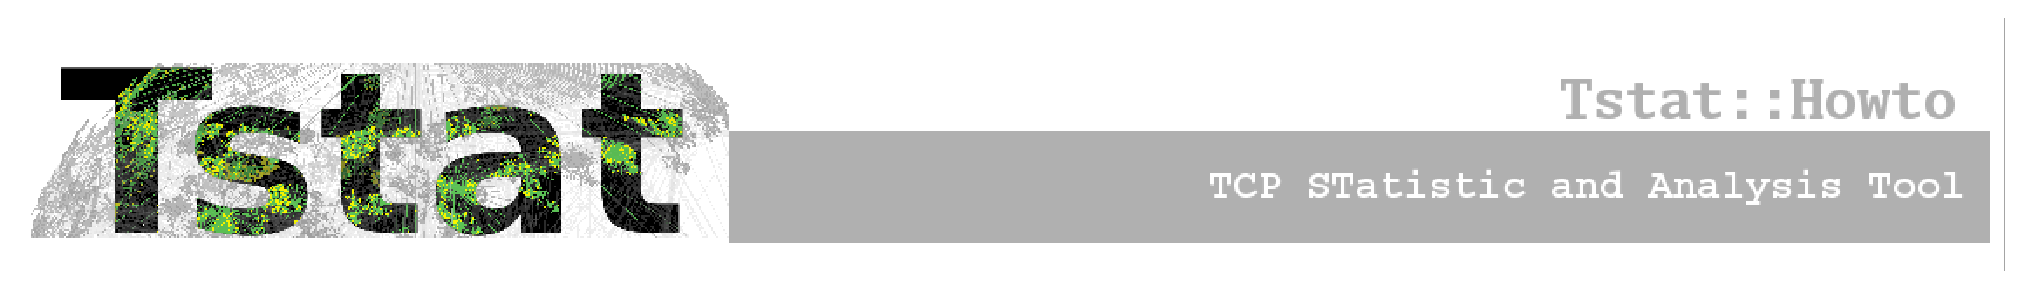
\includegraphics[width=\textwidth]{tstat_banner.eps}
\end{center}
\tableofcontents

%%  Latex generated from POD in document /orto/home14/munafo/devel/software/mplane/tstat3.0/doc/HOWTO/build/../HOWTO.pod
%%  Using the perl module Pod::LaTeX
%%  Converted on Fri Jun 26 12:04:20 2015

%%  Preamble supplied by user.

\clearpage

       %palatino
       \fontfamily{ppl}\selectfont


\section{Installation\label{Installation}\index{Installation}}


This document provides basic information
for the installation, configuration and usage 
of Tstat and the Bayesian framework for Skype
traffic identification.  A more general
description of the program as well as other
documentation can be found in the Tstat homepage
\textsf{http://tstat.tlc.polito.it}

\subsection{Requirements\label{Requirements}\index{Requirements}}
\subsubsection{Operating System\label{Operating_System}\index{Operating System}}


Tstat is tested on \texttt{Linux} systems (currently \texttt{Ubuntu}, \texttt{Debian}, \texttt{RedHat}, 
and \texttt{CentOS}, using \texttt{2.x} and \texttt{3.x} kernels), and on \texttt{Mac OS X} (starting 
from 10.6 \texttt{Snow Leopard} to the current 10.10 \texttt{Yosemite}). 
It includes support for compilation for \texttt{Android}, and has been reported working on 
\texttt{OpenWRT}. 
It should work under \texttt{FreeBSD}, \texttt{NetBSD}, and other \texttt{unix-like} systems, 
(although we don't have any of those platforms for testing purposes). 
If you are able to run Tstat on other OSes, we'll be happy to include them in the list.

\subsubsection{System Libraries\label{System_Libraries}\index{System Libraries}}


Tstat requires, by itself, a few library that should
already be installed on your system, such as 
\texttt{libpcap} (available from \textsf{http://www.tcpdump.org}) 
and the DAG drivers (available from \textsf{http://www.endace.com}), 
in case you use such hardware. With these libraries, 
you are ready to capture and process the traffic flowing
in your LAN.



Since Tstat might use pthread to improve the performance in case of real time
analysis, your system must support POSIX threads as well if you want to
profit of this feature. However, keep in mind that threaded execution 
is only an optional feature, and is necessary only for online traffic
analysis, so that this is not a strict requirement: for this reason,
threading is disabled by default.



Finally, to use the RRD functionalities, you also need to have a working
installation of RRDtool (available from \textsf{http://oss.oetiker.ch/rrdtool/}).

\subsection{Quick Install\label{Quick_Install}\index{Quick Install}}


Assuming that you want version \texttt{3.x.y}:

\begin{small}\begin{verbatim}
         wget http://tstat.polito.it/download/tstat-3.x.y.tar.gz
         tar -xzvf tstat-3.x.y.tar.gz
         cd tstat-3.x.y
         ./autogen.sh
         ./configure [--enable-libtstat] [--enable-zlib]
         make
         make install (with root privileges)
\end{verbatim}\end{small} \noindent
This commands install a executable file named \texttt{tstat} in \texttt{/usr/local/bin}.

\subsection{Complete control of Building\label{Complete_control_of_Building}\index{Complete control of Building}}


The most important elements in the Tstat's package are:

\begin{small}\begin{verbatim}
    tstat/
    tstat-conf/
    libtstat/
    include/
    libtstat-demo/
    doc/ 
    doc/HOWTO
    README AUTHORS NEWS INSTALL ChangeLog
\end{verbatim}\end{small} \noindent
The \texttt{tstat} directory contains the source code of Tstat which
is also the default building target. Beside Tstat it can also be compiled
the \texttt{Libtstat}, a shared library which allows to an external program to access 
to the traffic analysis functions of Tstat. In the \texttt{include} directory there is the
header file of the library instead in the \texttt{libtstat-demo} directory there is a simple 
program of example that shows how to use the Libtstat 
(see \textsf{Libtstat library} for more information about the Libtstat API).



The building of the Libtstat library is disabled by default but is provided
a configuration option to control this feature

\begin{small}\begin{verbatim}
    ./configure --enable-libtstat    # build tstat, libtstat and libtstat-demo
    ./configure                      # build only tstat
\end{verbatim}\end{small} \noindent
It is possible, if \texttt{Zlib} is found on the system, to compile Tstat to support the
direct creation of zlib compressed logs and dump files.

\begin{small}\begin{verbatim}
    ./configure --enable-zlib        # build tstat with zlib support
\end{verbatim}\end{small} \noindent
At the end of \texttt{configure} is printed a small report:

\begin{small}\begin{verbatim}
    -------------------------------------------------
      tstat Version 3.0
      -lpcap -lpthread -lm  -lrrd -lz
\end{verbatim}\end{small} \noindent
\begin{small}\begin{verbatim}
      Prefix: '/usr/local'
\end{verbatim}\end{small} \noindent
\begin{small}\begin{verbatim}
      Package features:
        - pcap      yes
        - zlib      yes
        - rrd       yes
        - libtstat  no
    -------------------------------------------------
\end{verbatim}\end{small} \noindent
This indicate if the libtstat has been selected or not for the building 
and if either \texttt{Librrd} or \texttt{Zlib} were found in the system, 
in which case they are automatically added in building the project.



Tstat's source code uses some preprocess definition to enable/disable some features,
like for example the DAG support which is disabled by default.
These definitions are declared in the \texttt{tstat/Makefile.conf} each with a specific 
description about its purpose so it should be easy change to behaviour in the building
process commenting/uncommenting some lines.

\begin{description}

\item[{}] \mbox{}

NB: remember to run \texttt{autoreconf} from the root of the package every time 
a change in these file is performed!!!

\end{description}


The building of Libtstat is separated from the building of Tstat so \texttt{libtstat/Makefile.conf}
file defines the set of option specific for the Libtstat, while \texttt{tstat/Makefile.conf}
is specific for Tstat.



In the directory \texttt{tstat-conf} there are some examples of configuration files 
needed by Tstat; for example the set of local addresses (-N option), 
the configuration of the histograms (-H), RRD tool (-R), runtime (-T) and 
bayesian framework (-B).



In the directory \texttt{doc} there are some plain text files that describes the format
of logs files generated by the analysis and in \texttt{doc/HOWTO} there is howto document 
in different file formats.
\texttt{README}, \texttt{AUTHORS}, \texttt{INSTALL}, \texttt{NEWS} and \texttt{ChangeLog} instead are plain files that
describes some general information about the package like the authors, the last new
features of the tools, etc...

\subsection{Complete control of Installation\label{Complete_control_of_Installation}\index{Complete control of Installation}}


The default \texttt{prefix} for installation is \texttt{/usr/local} so
Tstat executable in installed in \texttt{/usr/local/bin} and Libtstat 
is installed in \texttt{/usr/local/lib}. Anyway a different \texttt{prefix} can
be specified at configuration time

\begin{small}\begin{verbatim}
    ./configure --prefix=/absolute/path/where/install/tstat
\end{verbatim}\end{small} \noindent
Libtstat-demo is only a demonstration tool so is build only a local
executable that is not installed.



Libtstat is provided with \texttt{pkg-config} support so a \texttt{libtstat.pc} is installed in
\texttt{/usr/lib/pkg-config} and typing

\begin{small}\begin{verbatim}
    pkg-config --cflags --libs libtstat
\end{verbatim}\end{small} \noindent
it should appears an output like

\begin{small}\begin{verbatim}
    -I/usr/local/include  -L/usr/local/lib -lm -lpthread -lpcap -lrrd
\end{verbatim}\end{small} \noindent
that indicates the \texttt{CFLAGS} and \texttt{LIBS} options used in the building
process.

\section{Usage\label{Usage}\index{Usage}}


There are few things to know to run Tstat: first, you are required to have a
knowledge of the network that you want to monitor. 
Second, there are the few options that are described in this section.

\subsection{Synopsis\label{Synopsis}\index{Synopsis}}


Tstat primary usage is as a command-line tool; the synopsis of 
the command is the following:

\begin{small}\begin{verbatim}
    Usage:
        tstat [-htuvwpgSL0] [-d[-d]]
              [-s dir]
              [-N file]
              [-C file]
              [-Y file]
              [--keyvalue key | --keyfile file | --keybase64 file]                                                              
              [-W file]
              [-B bayes.conf]
              [-T runtime.conf]
              [-G globals.conf]                                   
              [-z file]
              [-A mask]
              [-H ?|file ]
              [-F file]                                           
              [-Z] [-P]
              [-r RRD_out_dir] [-R rrd_conf]
              [-l] [-i interface] [-E snaplen]
              [-f filterfile]
              <file1 file2>
\end{verbatim}\end{small} \noindent
\begin{small}\begin{verbatim}
    Options:
        -h: print this help and exit
        -t: print ticks showing the trace analysis progress
        -u: do not trace UDP packets
        -v: print version and exit
        -w: print [lots] of warning
        -c: concatenate the finput files
            (input files should already be in the correct order)
        -0: force the strict(er) privacy mode for logs
        -d: increase debug level (repeat to increase debug level)
\end{verbatim}\end{small} \noindent
\begin{small}\begin{verbatim}
        -s dir: puts the trace analysis results into directory
                tree dir (otherwise will be <file>.out)
        -N file: specify the file name which contains the
                 description of the internal networks.
                 This file must contain the subnets that will be
                 considered as 'internal' during the analysis.
                 Each subnet can be specified in one of the following types:
                 - <Network IP/NetMask> on a single line 
                     130.192.0.0/255.255.0.0
                 - <Network IP/MaskLen> on a single line 
                     130.192.0.0/16
                 - Pairs of lines with <Network IP> and <NetMask>
                     130.192.0.0
                     255.255.0.0
                 If the option is not specified all networks are
                 considered internal
\end{verbatim}\end{small} \noindent
\begin{small}\begin{verbatim}
        -M file: specify the file name which contains the
                 description of the MAC addesses that are to be considered internal.
                 MAC addresses must be in the 6 digit - hex notation.
                 Example:
                        11:22:33:44:55:66 
                        66:55:44:33:22:11 
                 If this option is specified, the -N param is ignored.
\end{verbatim}\end{small} \noindent
\begin{small}\begin{verbatim}
        -C file: specify the file name which contains the
                 description of the cloud networks.
                 This file must contain the subnets that will be
                 considered as belonging to a specific group of networks
                 (cloud) during the analysis.
                 Subnets are specified like in the -N option.
\end{verbatim}\end{small} \noindent
\begin{small}\begin{verbatim}
        -Y file: specify the file name which contains the
                 description of the encrypted networks.  
                 This file must contain the subnets for which the IPv4 address
                 will be anonymized using the Crypto-PAn algorithm.            
                 Subnets are specified like in the -N option.
\end{verbatim}\end{small} \noindent
\begin{small}\begin{verbatim}
        --keyvalue key: specify a string to be used as the key for address
                 anonymization.                                           
                 Valid only if the -Y option is also specified. Only one option
                 among --keyvalue, --keyfile, and --keybase64 can be used.
\end{verbatim}\end{small} \noindent
\begin{small}\begin{verbatim}
        --keyfile file: specify the file name which contain the plain text key
                 for address anonymization.                                   
                 Valid only if the -Y option is also specified. Only one option
                 among --keyvalue, --keyfile, and --keybase64 can be used.
\end{verbatim}\end{small} \noindent
\begin{small}\begin{verbatim}
        --keybase64 file: specify the file name which contain the Base64 encoded
                 key for address anonymization.                                 
                 Valid only if the -Y option is also specified. Only one option 
                 among --keyvalue, --keyfile, and --keybase64 can be used.
\end{verbatim}\end{small} \noindent
\begin{small}\begin{verbatim}
        -W file: specify the file name which contains the
                 description of the whitelisted hosts/networks.
                 This file must contain the subnets for which the IPv4 address
                 will be whitelisted and *NOT* anonymized using the Crypto-PAn algorithm.
                 Subnets are specified like in the -N option.                            
                 Meaningful only if the -Y option is also specified.
\end{verbatim}\end{small} \noindent
\begin{small}\begin{verbatim}
        -H ?: print internal histograms names and definitions
        -H file: Read histogram configuration from file
                 file describes which histograms tstat should collect
                 'include histo_name' includes a single histogram
                 'include_matching string' includes all histograms
                 whose name includes the string
                 special names are:
                 'ALL' to include all histograms
                 'ADX' to include address hits histogram
                 for example, to include all TCP related
                 and the address hits histograms, file should be:
                 include ADX
                 include_matching tcp
                 'adx_mask N' is a special command to define the 
                 size of the netmask used to aggregate the address histograms
                 (e.g. 'adx_mask 24' to use the 255.255.255.0 mask)
\end{verbatim}\end{small} \noindent
\begin{small}\begin{verbatim}
        -g: Enable global histo engine
        -S: No histo engine: do not create histograms files 
        -L: No log engine: do not create log_* files 
        -1: Use old (v1) log_mm format
        -B Bayes_Dir: enable Bayesian traffic classification
                      configuration files from Bayes_Dir
        -T runtime.conf: configuration file to enable/disable dumping
                         of traces and logs at runtime
        -G globals.conf: configuration file to provide at startup new values
                         to the internal global configuration constants     
        -z file: redirect all the stdout/stderr messages to the file specified
        -A mask: enable XOR-based anonymization for internal IPv4 addresses.
                 'mask' is a decimal, octal, or hexadecimal value.
        -X: disable the DN-Hunter DNS engine 
        -F file: specify the file name which contains the
                 list of DNS domains to be included/excluded from the
                 TCP traffic dump. Activated in the runtime configuration (-T)
        -Z: Create gzip compressed (.gz) log files.
        -P: Create gzip compressed (.gz) pcap dump files.
        -R conf: specify the configuration file for integration with
                 RRDtool. See README.RRDtool for further information
        -r path: path to use to create/update the RRDtool database
        -l: enable live capture using libpcap
        -i interface: specifies the interface to be used to capture traffic
        -E snaplen: specifies the snaplen size used to capture traffic.
                    It might be overridden by the interface slen size
        -f filterfile: specifies the libpcap filter file. Syntax as in tcpdump
\end{verbatim}\end{small} \noindent
\begin{small}\begin{verbatim}
        file: trace file to be analyzed
              Use 'stdin' to read from standard input.
\end{verbatim}\end{small} \noindent
\begin{small}\begin{verbatim}
    Note:
        When tstat is called with no arguments (on the command line),
        it will first check if a file <tstat.conf> is provided in the
        same directory where the execution started.
        In the latter case, arguments will be read from <tstat.conf>
        rather than from the command line
\end{verbatim}\end{small} \noindent
\begin{small}\begin{verbatim}
    Supported Input File Formats:
        tcpdump          tcpdump format -- Public domain program from LBL
        snoop            Sun Snoop format -- Distributed with Solaris
        etherpeek        etherpeek format -- Mac sniffer program
        netmetrix        Net Metrix format -- Commercial program from HP
        ns               ns format - Network simulator ns2 from LBL
        netscout         NetScout Manager format
        erf              Endace Extensible Record format
        tcpdump live     Live capture using pcap/tcpdump library
\end{verbatim}\end{small} \noindent
\subsection{Live Capture vs Trace Analysis\label{Live_Capture_vs_Trace_Analysis}\index{Live Capture vs Trace Analysis}}


Tstat can sniff and analyze traffic on-line through the
use of either the \texttt{libpcap} library or Endace DAG cards. 
The use of Tstat is very easy, especially if you have
experiences with \texttt{tcpdump}, although \texttt{tcpdump}'s knowledge
is not required to profitably use Tstat. Moreover, advanced 
users will enjoy the ability of on-line processing of traffic
captured with DAG cards.



As a minimal configuration, you must describe your network to Tstat. Indeed, in
order to distinguish forward and backward paths, Tstat needs to know which host
IP addresses can be considered as ``internal'' to the monitored network. 
There are three different format to specify the internal subnets and
if, for example, we use Politecnico di Torino subnets, which are \texttt{130.192.0.0/16} and
\texttt{192.204.134.0/24}, we can choose to use one of the following formats:

\begin{description}

\item[{$<$Network IP/MaskLen$>$ on a single line}] \mbox{}\begin{small}\begin{verbatim}
    130.192.0.0/16
    192.204.134.0/16
\end{verbatim}\end{small} \noindent
\item[{$<$Network IP/NetMask$>$ on a single line}] \mbox{}\begin{small}\begin{verbatim}
    130.192.0.0/255.255.0.0
    192.204.134.0/255.255.0.0
\end{verbatim}\end{small} \noindent
\item[{(only for backward compatibility) pairs}] \textbf{of lines with $<$Network IP$>$ and $<$NetMask$>$}\begin{small}\begin{verbatim}
    130.192.0.0
    255.255.0.0
    192.204.134.0
    255.255.0.0
\end{verbatim}\end{small} \noindent
\end{description}


Note that formats can be mixed in the configuration file and comment lines
can be specified using \texttt{'\#'} so using following
configuration is still correct

\begin{small}\begin{verbatim}
    # this is a comment
    130.192.0.0/24
    192.204.134.0/255.255.0.0
    192.168.0.0
    255.255.0.0
\end{verbatim}\end{small} \noindent
In the directory \texttt{tstat-conf} are placed the two files \texttt{net.all} and
\texttt{net.private}

\begin{small}\begin{verbatim}
    >cat tstat-conf/net.all
    # Mask to indicate that all IP subnets are supposed to be internal
    # The same result is obtained omitting the -N option
    0.0.0.0/0.0.0.0
\end{verbatim}\end{small} \noindent
\begin{small}\begin{verbatim}
    >cat tstat-conf/net.private
    # Example mask to consider as internal all the subnets in the 
    # 198.168. private addresses range
    192.168.0.0/16
\end{verbatim}\end{small} \noindent
that can be useful for generic elaborations. In any case, if the \texttt{-N} option
is not specified all networks are considered internal.



We can now run Tstat to capture the traffic flowing across 
our network, with the following command, which must be run as \texttt{root} (as you
need to capture packets by putting the Ethernet interface in promiscuous mode).
The simplest command is the following:

\begin{small}\begin{verbatim}
         ./tstat -l -N net.conf
\end{verbatim}\end{small} \noindent
Beside live-capture, it is possible to run Tstat on a previously collected 
trace file, where the trace format can be any of the following:

\begin{small}\begin{verbatim}
        Supported Input File Formats:
                tcpdump          tcpdump -- Public domain program from LBL
                snoop            Sun Snoop -- Distributed with Solaris
                etherpeek        etherpeek -- Mac sniffer program
                netmetrix        Net Metrix -- Commercial program from HP
                ns               ns -- network simulator from LBL
                netscout         NetScout Manager format
                erf              Endace Extensible Record Format
                DPMI             Distributed Passive Measurement Interface (DPMI) format
                tcpdump live     Live capture using pcap/tcpdump library
\end{verbatim}\end{small} \noindent
Tstat will try to read trace files given as input, and to automatically identify
the correct dump format. Trace files can be compressed or uncompressed, and
Tstat will automatically detect the compression tool used (supported formats are
\texttt{compress, gzip, bzip2, 7z}).



Without loss of generality, we assume to use the first of the above formats. The
calling syntax is similar to the previous one, with the exception of the absence
of the live-capture switch \texttt{-l} and the presence of the name(s) of the file(s)
that have to be processed. For example, the following command can be used to
analyze a trace file named \texttt{LAN.dump.gz}. Results of the analysis
will be stored in a subdirectory named \texttt{trace1}; as before, \texttt{net.conf} contains  the
subnet description that will be considered as ``internal'' during the
analysis.

\begin{small}\begin{verbatim}
         ./tstat -s trace1 -N net.conf LAN.dump.gz
\end{verbatim}\end{small} \noindent
\subsection{More Control\label{More_Control}\index{More Control}}


We can control the interface that we want to sniff from as well as
the output directory name as follows:

\begin{small}\begin{verbatim}
         ./tstat -i eth1 -l -s test -Nnet.conf
\end{verbatim}\end{small} \noindent
Moreover, we can also pipe Tstat input using the special keyword
\texttt{stdin} as input, as in the following command (piping ns2 output to 
Tstat is left as an exercise for the reader):

\begin{small}\begin{verbatim}
         tcpdump -s 80 -i eth0 -w - ip | ./tstat -Nnet.conf -spiped stdin
\end{verbatim}\end{small} \noindent
In this case, Tstat is fed by \texttt{tcpdump}'s output, and the latter has been
instructed to capture packets on the eth0 device, collecting the
first 80 bytes (to track uniquely packet headers) of IP packets only, 
and send the output to \texttt{stdout}. Moreover, since Tstat understands 
the \texttt{libpcap} syntax, filters can be stored in text files, as in 
the following command sequence:

\begin{small}\begin{verbatim}
         echo "vlan and ip and host 10.0.0.1" > tcpdump.conf
         ./tstat  -i eth0 -l -f tcpdump.conf -N net.conf -s filtered
\end{verbatim}\end{small} \noindent
\subsection{Process Signalling\label{Process_Signalling}\index{Process Signalling}}


While Tstat runs, it is possible to interact with the program using Unix signals. 
This might be useful if Tstat is executed unsupervised, or without full terminal control 
(redirecting stdout/stderr using the \texttt{-z} option).



Currently Tstat reacts to the \texttt{USR1} and \texttt{INT} signals.



Sending a \texttt{USR1} signal to a running ‘Tstat’ process makes it print the current flow 
statistics to standard error and then resume its operations.



Sending a \texttt{INT} signal to a running ‘Tstat’ process makes it gracefully terminate its 
operations, writing all the statistics to the output files, flushing and closing the files, and
printing the overall flow statistics to stderr before exiting. This is equivalent to interrupting
the program pressing \texttt{Ctrl-C} from the control terminal.



If Tstat is running unsupervised, you should avoid terminating the process using the \texttt{KILL} signal
( \texttt{'signal -KILL'} or \texttt{'signal -9'}), since it will possibly leave the log files in an 
inconsistent state, and you should therefore use either the \texttt{INT} or the \texttt{TERM} signals
 (\texttt{'signal -INT'} or \texttt{'signal -TERM'}).

\section{Output\label{Output}\index{Output}}


Tstat collects several network-layer as well as transport-layer measurements,
which are described in full details in \textsf{http://tstat.polito.it/measure.shtml}.
As output, Tstat produces four different types of files: histograms, round robin database, 
packet level traces and other plain text logs.



By default Tstat collect all the output results in a directory with the same name of the input 
trace appending the suffix \texttt{.out} or \texttt{stding} in case of a live capture:

\begin{small}\begin{verbatim}
    ./tstat -N net.conf trace1.pcap trace2.pcap # output dir: trace1.pcap.out, trace2.pcap.out
    ./tstat -N net.conf -li eth0                # output dir: generate stdin   
    ./tstat -N net.conf -s trace1 trace1.pcap   # output dir: trace1
\end{verbatim}\end{small} \noindent
In any case, inside the output directory is generated a subdirectory named with the
timestamp of the first packet analyzed and inside this directory the files generated
are organized as follow:

\begin{small}\begin{verbatim}
    <output_root>
    `-- 23_00_28_Jun_2008.out
        |-- 000
        |   `--- histo_logs
        |-- 001
        |   `--- histo_logs
        ...
        |-- LAST
        |   `--- histo_logs
        |
        |-- traces00
        |   `--- dump_traces
        |-- traces01
        |   `--- dump_traces
        ...
        `-- other_logs
\end{verbatim}\end{small} \noindent
This means that the RRD output files are not collected inside the output directory, 
in fact there is a specific command line option (-r) to indicate where this results 
have to be placed.



Recall that Tstat assumes that traces are collected on a bidirectional link,
such that both data and control packets belonging to the same flow are observed;
with the help of the figures below, we will explain the different classification
of measurements used by Tstat.



         \begin{figure}[!htb]
             \begin{center}
                 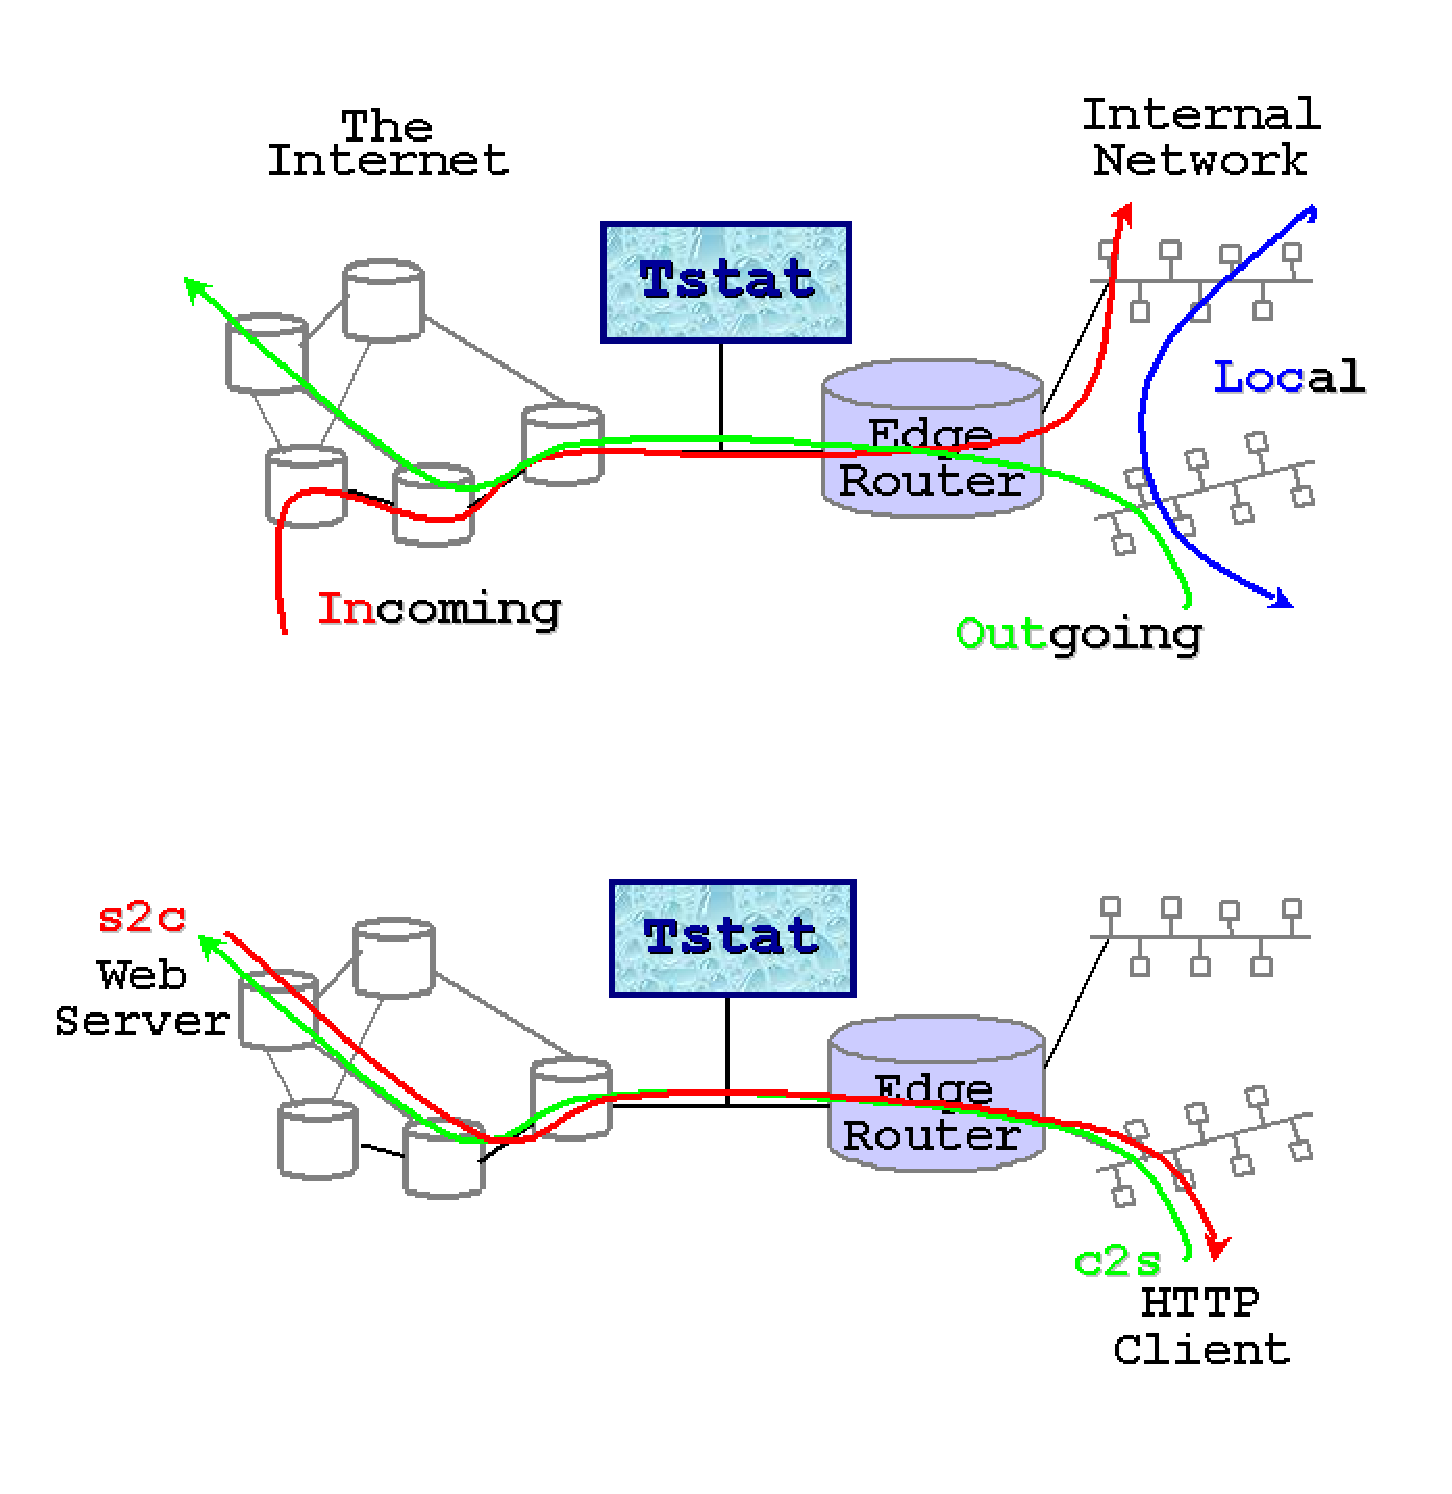
\includegraphics[width=0.6\textwidth]{tstat_output.eps}
             \end{center}
         \end{figure}





Tstat identifies hosts based on their IP address. Given the description
of the internal hosts through the \texttt{-N} command line option, Tstat
distinguishes among \textit{incoming}, \textit{outgoing} and \textit{local} 
measurements. Packets whose destination is an internal host and whose source is
an external host will contribute to \textit{incoming} measurements (red arrow in the
top figure), whereas packets going
in the opposite direction will contribute to \textit{outgoing} measurements (green
arrow in the top figure). Finally, in
some cases it is possible that Tstat observes packets whose source and
destination host belong to the internal host set: in such cases, measurements
will be classified as \textit{local} (blue arrow in the top figure).
Notice that packets whose source and destination IP
addresses belong to the external host set will be discarded.
For example, consider a setup in which Tstat is attached to a snoop port of a
LAN switch. Then Tstat will be fed by i) \textit{outgoing} packets going to the default gateway,
ii) \textit{incoming} packets coming from the default gateway, iii) \textit{local} packets.



Note that if you either do not know or do not want to distinguish between
internal, external and local hosts, you may enable the \texttt{-DLOG\_UNKNOWN} 
(in \texttt{tstat/Makefile.conf} or \texttt{libtstat/Makefile.conf})
directive when compiling. Tstat will then be less strict, but results may
be difficult to be correctly interpreted.



Considering instead the \textit{role} of the host that sent the packet, statistic are
collected distinguishing between \textit{clients} (green arrow in the bottom figure)
and \textit{servers} (red arrow in the top figure), i.e., host
that opens a connection and and host that replies to connection request. Recall
that while TCP connections are well defined, UDP (and RTP/RTCP) connection
definition is more fuzzy. In this latter case, Tstat will consider as client the
source IP address of the host that sent the first packet of that flow, while the
server will be the host identified by the destination IP address of the same
packet.



Therefore, when applicable, Tstat will keep track of measurements referring to
the same measured quantity by \textit{appending} a specific tag (see Sec.~\ref{Histograms}) or using a \textit{flag} 
(see \emph{Logs}).

\subsection{Logs\label{Logs}\index{Logs}}


Tstat creates a set of TXT flow files in the main output directory: \texttt{log\_tcp\_complete},
\texttt{log\_tcp\_nocomplete}, \texttt{log\_udp\_complete}, \texttt{log\_mm\_complete}, \texttt{log\_video\_complete},
\texttt{log\_skype\_complete}, \texttt{log\_chat\_complete} and \texttt{log\_chat\_messages}.
TCP flows can be either completed or not depending whether Tstat observed the
3-way handshaking or not; in the first case, all the measured indexes relatively
to each flow will be collected in the \texttt{log\_tcp\_complete}; in the latter
case,  flows are considered as garbage and stored in \texttt{log\_tcp\_nocomplete};
Similarly, a complete log keeping track of each UDP flow measured indexes is
maintained in the \texttt{log\_udp\_complete} file. Being UDP basically a
connectionless protocol, it is impossible to distinguish among \texttt{complete} and
\texttt{nocomplete} flows in this case.



Furthermore the following log files are created: \texttt{log\_video\_complete} and
\texttt{log\_streaming\_complete} for TCP video 
streaming flows (i.e. RTMP or HTTP-based video services like YouTube), 
\texttt{log\_mm\_complete} for multimedia flows
(i.e. RTP, RTCP, etc), \texttt{log\_chat\_complete} for IM protocols (i.e. MSN, Jabber, etc) and
\texttt{log\_skype\_complete} for Skype traffic.



Description of the file format of each log file can be found in
\textsf{http://tstat.polito.it/measure.shtml}.



If Tstat has been compiled with Zlib support, it will directly create gzip compressed 
logs (.gz) when the command line option \texttt{-Z} is used. Internal compression might be 
CPU demanding: before enabling it, you should consider its possible effects on the Tstat 
performance.

\subsection{Histograms\label{Histograms}\index{Histograms}}


Histograms are generated periodically to generate the \textit{distribution} of a 
given quantity within a time interval. Tstat collects all the
measurement data during a given measurement interval defined by the \texttt{MAX\_TIME\_STEP} 
parameter, which is hard-coded in the \texttt{tstat/param.h} file to 5 minutes. Please, note
that changing the \texttt{MAX\_TIME\_STEP} parameter may affect RRD creation as well.
For example, considering the IP packet length, Tstat updates, for
each observed IP packet, the counter of the number of observed packets with a
particular length. At the end of the measurement period, Tstat then saves
the values stored in the histogram in a subdirectory named with a incrementally counter
of three digits, resets all the internal values, and then restarts 
the samples collection.



To separate statistics respecting the verse (input, output or local) and the role of a
peer in the communications, is appended a tag to files generated:

\begin{description}

\item[{\texttt{\_out}}] \mbox{}

outgoing: from an internal host to an external host


\item[{\texttt{\_in}}] \mbox{}

incoming: from an external host to an internal host


\item[{\texttt{\_loc}}] \mbox{}

local between two internal hosts


\item[{\texttt{\_c2s}}] \mbox{}

going from the Client to the Server


\item[{\texttt{\_s2c}}] \mbox{}

going from the Server to the Client

\end{description}


Considering the last example of previous section, we run:

\begin{small}\begin{verbatim}
         ./tstat -s trace1 -N net.conf 23_00_28_Jun_2008.dump.gz
\end{verbatim}\end{small} \noindent
The output generated by Tstat consists of a directory tree like the following:

\begin{small}\begin{verbatim}
        trace1
    `-- 23_00_28_Jun_2008.out
        |-- 000
        |   |-- addresses<tag>
        |   |-- flow_number<tag>
        |   |-- ip_len_in<tag>
        |    ...
        |   |-- udp_port_flow_dst<tag>
        |   `-- udp_tot_time<tag>
        |-- 001
        |   |-- addresses<tag>
        |   |-- flow_number<tag>
        |   |-- ip_len_in<tag>
        |    ...
        |   |-- udp_port_flow_dst<tag>
        |   `-- udp_tot_time<tag>
        ...
        |-- LAST
        |   |-- addresses<tag>
        |   |-- flow_number<tag>
        |   |-- ip_len_in<tag>
        |    ...
        |   |-- udp_port_flow_dst<tag>
            `-- udp_tot_time<tag>
\end{verbatim}\end{small} \noindent
Subdirectories with increasing numbers will be created for each measurement
period with the format \texttt{nnn/}; histograms collecting measurement results will
be created in these directories; note that the histograms referring to the last
\textit{partial} time period will be stored in the LAST subdirectory. The option \texttt{-g}
adds also the subdirectory GLOBAL containing the global histograms for the whole
measurement period.



The \texttt{-H} has to be used to enable the histogram engine, specifying a configuration
file of \texttt{?} to have a complete list of the available histograms. The syntax of
the configuration file is really simple:

\begin{small}\begin{verbatim}
    include ALL             # add all histograms
    include ADX             # histogram to count how many times ip address are used
    adx_mask 16             # define the size of the netmask for the ADX histogram
\end{verbatim}\end{small} \noindent
\begin{small}\begin{verbatim}
    include ip_len_in      # histogram of the ip packet length of the input traffic
\end{verbatim}\end{small} \noindent
\begin{small}\begin{verbatim}
    include_matching ip_    # match all the histograms which name start with 'ip_'
\end{verbatim}\end{small} \noindent
Histogram data are saved using simple ASCII files: 
the first line contains a description of the
measured quantity, while the second line contains the parameters of the histograms
(minimum and maximum values, and size of each bins). The list of all
the counter index and values is then dumped. To limit the file size, the
corresponding entry is omitted if the counter is zero.
For example, the histogram of the packet length \texttt{ip\_len\_in} looks like:

\begin{small}\begin{verbatim}
     #IP packet length - incoming packets
     #min=0 bin_size=4 max=1600
     28 7
     36 277
     40 11760
     44 3463
     ...
\end{verbatim}\end{small} \noindent
Simple \textsf{Post Processing} tools are available to automatically manage the histogram
database.

\subsection{RRD\label{RRD}\index{RRD}}


The RRD output consists of a series of binary files stored in the RRD format.
Tstat forces a particular \textit{naming notation} of such files, which follows
the configuration rules described later in Sec.~\ref{RRD_Configuration}.



The RRD can then be queried with the standard RRDtool commands, such as
\texttt{rrdcreate}, \texttt{ rrdupdate},  \texttt{ rrdgraph}, \texttt{ rrddump}, \texttt{ rrdfetch}, 
\texttt{ rrdtune}, \texttt{ rrdlast}, \texttt{ rrdxport}, to whose manual pages we refer 
the reader for further informations.

\subsection{Packet Level Traces\label{Packet_Level_Traces}\index{Packet Level Traces}}


Inside Tstat there is a \texttt{Deep Packet Inspector - DPI} which is able to identify
traffic communications at application level looking the composition of the payload
of packets.



This feature is controlled by the \textsf{Runtime module} and the output
files are placed in subdirectories named \texttt{tracesNN} where \texttt{NN} is an counter
incremented every time the runtime configuration is changed.
In any case, for each configuration, the input traffic in 
is splitted in traces with windows of 1 hour, that is, for example,
if we start the dump at 9:00 am

\begin{small}\begin{verbatim}
    traces00/udp_complete.pcap0       #all the udp traffic from 9:00  to 10:00
    traces00/udp_complete.pcap1       #all the udp traffic from 10:00 to 11:00
    ...
\end{verbatim}\end{small} \noindent
All the traces are in \texttt{pcap} format and, because of the level 2 headers are in
general useless for statistic purpose, each packet dumped is composed of a bogus
Ethernet header (contains only zeros expect for the \texttt{type} field which is IP)
followed by the original packet starting from IP header. The input packets
can also be truncated after a specific amount of bytes which can be configured
using the \texttt{snap\_len} specific option in the configuration file.



If Tstat has been compiled with Zlib support, it will directly create gzip compressed 
traces (.pcap.gz) when the command line option \texttt{-P} is used. Internal compression 
of the packet traces is highly CPU demanding: before enabling it, you should consider 
its possible effects on the Tstat performance.

\subsection{Privacy concerns\label{Privacy_concerns}\index{Privacy concerns}}


To cope with privacy concerns and possible legal requirements, Tstat has a few options
to mitigate the user information exposed in the log files.



One main privacy concern is the presence of the actual user IP addresses in logs.
To hide this information, Tstat implements two possible solutions.



The first one is a simple XOR-based obfuscation of the IP address, activated by the 
command line option \texttt{-A mask}. The 32-bit mask is applied \textbf{only} to internal IPv4 
addresses, as defined by either the \texttt{-N} or the \texttt{-M} command line options. If no 
internal network is defined, all IPs are considered internal and they are all 
obfuscated, reducing the usefulness of the logs to identify well known services.
The XOR-based obfuscation is applied as soon as the IP datagram is parsed, so
any saved packet level trace will contain the obfuscated IP addresses.



The second solution is a complex cryptographical anonymization of the IP addresses,
based on the well known Crypto-PAn[*] algorithm.
Crypto-PAn is a prefix-preserving IP anonymizer, and it is activated providing a 
list of IP networks to be anonymized using the command line option \texttt{-Y}. 
The networks are indicated in a format similar to the one used for the \texttt{-N} and \texttt{-C}
command line options. Any IPv4 address matching one of those networks is marked for 
encryption. Since the anonymization operations are CPU-intensive, any IP address 
is anonymized only once, the translation cached, and it is actually used only when the 
IP address must be printed in the logs. 
Since the original IP address is still used internally by Tstat and the translation is 
only used when printing the logs, any saved packet level trace will contain the 
\textbf{original non encrypted} IP addresses.
It is possible indicate a list of IP addresses and networks to be excluded from the 
encryption process using the \texttt{-W} command line option with a file in the same format 
used for the \texttt{-N} option. Addresses satisfying both the \texttt{-Y} and the \texttt{-W} lists 
will be whitelisted and will appear \textbf{unencrypted} in the log files.



The encrytion key used by the Crypto-PAn algorithm can be provided either directly on 
the command line, using the \texttt{--keyvalue} option, or from a file, using 
either the \texttt{--keyfile} or the \texttt{--keybase64} options. The \texttt{--keyfile} option
can be used for a plain text ASCII key, while the \texttt{--keybase64} option will treat 
content as a Base64 encoded key, so its suitable for an encoded binary key. In any case
the key is supposed to be 32 bytes long: longer keys are truncated to 32 bytes, and 
shorter keys are padded with zeros. If no key is provided, a key is generated reading 
32 random bytes read from \texttt{/dev/random}, so it will change every time Tstat starts.
Due to the blocking nature of \texttt{/dev/random}, it might take some time for Tstat to
start if there is not enough entropy on the system random generator.



The key used in each Tstat session is always saved in Base64 format in a file named 
\emph{CPanKey\_$<$datetime}$>$  (where \textit{datetime} is the current time of the day) that is 
created in the log directory root (the one indicated by the \texttt{-s} command line option).
The generated file is suitable to be later used as the argument of the \texttt{--keybase64} 
option.



Only IPv4 address are obfuscated or anonymized. There is currently no support in Tstat
for IPv6 anonymization, and obfuscation of TCP/UDP port numbers is of limited usage in
a traffic analysis tool such as Tstat.
Obfuscated (\texttt{-A}) addresses are not explicitely indicated in the log files (if they are
internal, and obfuscation was active, they are actually obfuscated). The presence of 
anonymized (\texttt{-Y}) address is explicitely indicated in the log files in the \texttt{c\_iscrypto}
and \texttt{s\_iscrypto} columns.
The \texttt{-A} and \texttt{-Y} options are not mutually exclusive, so it is possible to obfuscate the
internal addresses and, at the same time, anonymize another, possible overlapping, set of
IP addresses.



Beside the privacy issues related to the IP addresses, logs contain information that 
might be considered sensitive, i.e. the URLs information in \texttt{log\_http\_complete} and 
the YouTube VideoIDs in \texttt{log\_video\_complete}. The command line option \texttt{-0} make Tstat 
run in privacy mode: in this mode, the runtime.conf option \texttt{httplog\_full\_url} is forced 
to 0, so that full URLs cannot be logged in \texttt{log\_http\_complete}, and the YouTube 
Video IDs in \texttt{log\_video\_complete} are masked as \texttt{'XXX'}.



[*] \textsf{http://www.cc.gatech.edu/computing/Telecomm/projects/cryptopan/}

\subsection{Post Processing\label{Post_Processing}\index{Post Processing}}


This section could be a separate HOWTO, since this
argument cannot be treated exhaustively. Perl, Awk, Ruby
\textit{Your-Favorite-Scripting-Language} scripts are definitively
best candidates to post-process \texttt{log\_*} files.



In the Tstat download page and in the source archive, you
can find \texttt{plot\_time.pl} and \texttt{plot\_cum.pl}, two Perl scripts that may be useful
to produce either i) time or ii) aggregated plots over different time spans.
They directly access the histogram database created by Tstat.
Please, refer to \textsf{http://tstat.polito.it/software.php\#postprocess}.



In the source code, in \texttt{scripts/MySQL/}, you can also find a few Perl 
scripts to load the main \texttt{log\_*} files in a simple MySQL database, for further 
post-processing.



RRD files can be manipulated to obtain \textit{indirect} 
metrics through the RPN manipulations mechanism provided 
by RRDtool.

\subsection{Storage Considerations\label{Storage_Considerations}\index{Storage Considerations}}


To give the user a rough idea of the size of the output,
let us consider a 6 hours long, 1.6GB packet-level trace containing 
21M packets, sniffed with \texttt{tcpdump} that was used throughout this tutorial.
Tstat identified and analyzed about 729K flows, of which about 495K were 
TCP flows, trashing 20K of them into \texttt{log\_nocomplete}.
Referring to the Sec.~\ref{Output} above shown,
we can express the following observations:

\begin{description}

\item[{Histogram}] \mbox{}

As previously described, in order to take into account the flow directions,
several histograms are dumped for the same variable \texttt{var\_\{in,out,loc,c2s,s2c\}}.
Currently, about 60 measurement indexes, described in 
\textsf{http://tstat.tlc.polito.it/measure.shtml},  are logged, for a total
of 180 files. Each of the \texttt{000/}, \texttt{001/} ... \texttt{LAST/} directories is about
500KB-1MB depending on the network traffic and on the file system block
allocation mechanism.



Therefore,  as a rule of thumb, you can count about 1MB of storage due to
histograms every 5 minutes of traffic (independently of the amount of actual
traffic load during the 5 mins...). This can be useful in order to set the
periodic dump timer to the desired trade off among time granularity versus
storage size  required.


\item[{RRD}] \mbox{}

The \texttt{rrd/} directory is, per construction, of fixed size: this should not be a
surprise, since this is the goal of RRD. Therefore, the size of the database
does not depend on the amount of network traffic processed, but rather on the
RRD configuration. For the standard configuration supplied with Tstat, which is
also the one used in our Web server, the whole database occupy only 6MB and
consists of about 250 files.


\item[{Logs}] \mbox{}

The total size of the log files amount to about 200MB, which 
gives  a 8x reduction factor w.r.t. the packet-level trace; or,
the storage cost of each flow is about 400 bytes.



Note that the \texttt{log\_*} can be further compressed, using the \texttt{-Z} Tstat
command line option or \texttt{gzip} to less than 50MB, which gives a further 
4x size gain; however, for a matter of performance, is preferable 
to compress the log files \textit{offline}.

\end{description}


Finally, consider that on a common PC architecture (specifically,
Intel P4 2.40GHz equipped with 2GB of RAM and 7200rpm hard-disk),
the whole trace elaboration took only 4 minutes; thus, the 
analysis rate is roughly 85Kpkts/sec or 3Kflows/sec.

\section{RRD Module\label{RRD_Module}\index{RRD Module}}
\subsection{RRDtool Installation\label{RRDtool_Installation}\index{RRDtool Installation}}


In order to get Tstat RRD module working, you will need to install RRDtool first
(refer to the homepage of RRDtool \textsf{http://oss.oetiker.ch/rrdtool/}  to accomplish this step).
The autoconf file \texttt{configure} of Tstat then should automatically add the RRD support 
if it find one (see Sec.~\ref{Complete_control_of_Building}).

\subsection{RRD Configuration\label{RRD_Configuration}\index{RRD Configuration}}


Tstat RRD configuration is very easy, being centralized
in a single text-file, which allows to specify at runtime what measurements
should be monitored. The operating frequencies
for the RRD sampling (i.e., the parameters for the temporal 
averages) are hard-coded into \texttt{rrdtool.h} and are chosen to 
mimic MRTG behavior. Again, take care that modifying the \texttt{MAX\_TIME\_STEP}
parameter may affect the RRD management as well.



The RRD configuration file, specified through the command line option \texttt{-R},
should contain one line for each of the Tstat parameters that have
to be integrated into a Round Robin Database. Each line allows to
specify which statistical properties of the variable has to be tracked,
as follows:

\begin{small}\begin{verbatim}
          tstat_var1 avg min max stdev var idx:e,f,g,h,other prc:i,j,k
\end{verbatim}\end{small} \noindent
where \texttt{avg,min,max,stdev,var,idx,prc,other} are keywords, whereas \texttt{i,j,k} 
are floating point numbers and \texttt{e,f,g,h} integer values; note that
the list of indexes (e.g., TCP ports), values (e.g., packet size)
and percentiles are comma separated. The name of the variables are
Tstat internal ones: they can be seen by executing \texttt{./tstat -H},
Alternatively, you can directly look into the \texttt{000/} ...  \texttt{LAST/}  directories or
or at \textsf{http://tstat.polito.it/measure.shtml}



Valid configuration lines are, e.g.:

\begin{small}\begin{verbatim}
          #
          # inspect IP packet length average, specific values and distribution
          #
          ip_len_in   avg prc:50,90,95,99 idx:40,1500,other
\end{verbatim}\end{small} \noindent
\begin{small}\begin{verbatim}
          #
          # TCP well known ports       
          #                       
          # 20    FTP-DATA             
          # 21    FTP                  
          # 22    SSH                  
          # 23    telnet               
          # 25    SMTP                 
          # 80    HTTP                 
          # ...                        
          #
          tcp_port_dst_in       idx:20,21,22,23,25,80,other
\end{verbatim}\end{small} \noindent
\begin{small}\begin{verbatim}
          #
          # good approximation of the distribution of the RTT,
          # taking into account only the incoming path contribution
          #
          tcp_rtt_avg_in  prc:0.1,1,5,10,25,50,75,90,95,99,99.9
\end{verbatim}\end{small} \noindent
where, evidently, the lines starting with a \texttt{\#} sign are treated as comments.
Our Web server is currently running with the configuration
available at \textsf{http://tstat.polito.it/download/rrd.conf}.



For each specified quantity defined in the rrd.conf file, a corresponding file
will be created.
For example, consider that the generic configuration line:

\begin{small}\begin{verbatim}
          tstat_var avg min max stdev var idx:e,f,g,h,other prc:i,j,k
\end{verbatim}\end{small} \noindent
will produce the following files (13 in total):

\begin{small}\begin{verbatim}
          tstat_var.{avg,min,max,stdev,var}.rrd
          tstat_var.idx{e,f,g,h,oth}.rrd
          tstat_var.prc{i,j,k}.rrd
\end{verbatim}\end{small} \noindent
\subsection{Tstat RRD and the Web\label{Tstat_RRD_and_the_Web}\index{Tstat RRD and the Web}}


From the Tstat web site, you can
download the most up-to-date version of \texttt{tstat\_rrd.cgi},
which is the CGI script that renders the Web interface.
Here is some basic tips to get it working; if you wonder
how to write your own graph templates, then you are probably
skilled enough to get it on your own \texttt{:)}

\subsubsection{Database Structure\label{Database_Structure}\index{Database Structure}}


The CGI scripts allow to browse on the fly the RRD database structure.
The \texttt{rrd\_data} directory is the root of the tree, where each
directory contains either i) other directories (i.e., is a box) 
or ii) a RRD-database, in which case the node is a leaf and will be
shown in the interface. In case that a directory is a plain box, it may
optionally contain some files (specifically 
\{\texttt{HEADER},\texttt{FOOTER},\texttt{README}\}.\{\texttt{html},\texttt{txt}\})
that will be rendered by \texttt{tstat\_rrd.cgi}. 
By default, the cgi script tries to load the html version;
otherwise, it tries to displays "$<$pre$>$ `cat FILE` $<$/pre$>$"
if such a FILE exists; finally, it will display a default message
held in \$default\{README\} hard coded in the script.



Here is an example of the rrd\_data directory which holds part of the RRD database
accessible from the Tstat web page.

\begin{small}\begin{verbatim}
        rrd_data/
         |-- Example
         |-- GARR
         |   |-- garr-live
         |   `-- garr-old
         `-- Polito
             |-- 2000
             |   |-- Apr
             |   |-- Jun
             |   |-- Jun,post155
             |   `-- May
             |-- 2001
             |   |-- Feb
             |   `-- Jan
             |-- 2005
             |   |-- Apr
             |   `-- Feb
             `-- Current
\end{verbatim}\end{small} \noindent
\subsubsection{Web Configuration\label{Web_Configuration}\index{Web Configuration}}


The web configuration really depends on your web server configuration. Few
dependencies are required, most notably, the RRD Perl library from the RRDtool
installation.



It is advisable to store the Tstat RRD files
everywhere you want, and then create a symbolic link 
named \texttt{rrd\_data} that points to it (i.e., to the root of 
the RRD database tree). Similarly for the directory
where the rendered images should be stored (defaults to \texttt{cgi-bin/rrd\_images})
and can be a symbolic link as well.
The names of these symbolic links can be redefined in the 
configuration section of \texttt{tstat\_rrd.cgi} if needed:

\begin{small}\begin{verbatim}
        #   ____________________________
        #  /                            \
        # /    configuration  __________/
        # \__________________/.:nonsns:.
        #
        # specify path to the root of the rrd database tree
        # by default, I assume there is a symbolic link in cgi-bin/
        # named rrd_data
        $RRD_DATA = 'rrd_data';
\end{verbatim}\end{small} \noindent
\begin{small}\begin{verbatim}
        # same thing for image directory
        # in my case, var/www/cgi-bin/rrd_images is
        # a symbolic link to "/var/www/html/rrd_images";
        # from the html browser's perspective
        $IMG_DIR = "rrd_images";
\end{verbatim}\end{small} \noindent
\section{Runtime Module\label{Runtime_Module}\index{Runtime Module}}


This module has been developed with the specific target to try to control the disk
occupation and to have a minimal interface
to execution process to enable/disable some feature without restarting it. 
In particular, the system controls two specific outputs: the writing of log files and packet level traces, so
is possible to disable the writing of logs (histograms, RRD and all the others) if they
became to bigs, and to dynamically change the set of packet level traces to collect.



The module works with simple polling system that is it periodically tests if a configuration file,
specified with the \texttt{-T} option when Tstat is executed, is changed from the previous check
and in this case, the new configuration replace the previous one.
The polling process is controlled by the global constants \texttt{Runtime\_Config\_Idle} and 
\texttt{Runtime\_Mtime\_Counter}, that can be overriden at startup with the \texttt{-G} option, as described
in the \textsf{Global Constants} section.



The configuration file has an \texttt{ini} file syntax:

\begin{small}\begin{verbatim}
    > cat tstat-conf/runtime.conf
    # print logs on disk
    [log]
    histo_engine = 0    # logs created by histogram engine
    rrd_engine = 0      # logs created by rrd engine
    log_tcp_complete = 0            # tcp connections correctly terminated
    log_tcp_nocomplete = 0          # tcp connections not properly terminated
    log_udp_complete = 0            # udp flows
    log_mm_complete = 0             # multimedia 
    log_skype_complete = 0          # skype traffic
    log_chat_complete = 0           # MSN/Yahoo/Jabber chat flows
    log_chat_messages = 0           # MSN/Yahoo/Jabber chat messages
    log_video_complete = 0          # video (YouTube and others)
    log_http_complete = 0           # all the HTTP requests/responses
\end{verbatim}\end{small} \noindent
\begin{small}\begin{verbatim}
    # log options
    [options]
    tcplog_end_to_end = 0       # End_to_End set of measures (RTT, TTL)
    tcplog_layer7 = 0           # Layer7 set of measures (TLS cert., message counts)
    tcplog_p2p = 0              # P2P set of measures (P2P subtype and ED2K data)
    tcplog_options = 0          # TCP Options set of measures
    tcplog_advanced = 0         # Advanced set of measures
    httplog_full_url = 0        # Partial (=1) or full (=2) URLs in log_http_complete
\end{verbatim}\end{small} \noindent
\begin{small}\begin{verbatim}
    videolog_end_to_end = 0     # TCP End_to_End set of measures (RTT, TTL)
    videolog_layer7 = 0         # Layer7 set of measures (TLS cert., message counts)
    videolog_videoinfo = 0      # Additional video info (resolution, bitrate)
    videolog_youtube = 0        # YouTube specific information
    videolog_options = 0        # TCP Options set of measures
    videolog_advanced = 0       # Video-related Advanced mesurements (rate)
\end{verbatim}\end{small} \noindent
\begin{small}\begin{verbatim}
    # protocols to dump
    [dump]
    snap_len = 0        # max num of bytes to dump from ip hdr (included)
                        # 0 == all bytes
    slice_win = 0       # dimension (in secs) of the dumping window
                        # used to slice the input traffic in different traces
                        # 0 == no slicing
\end{verbatim}\end{small} \noindent
\begin{small}\begin{verbatim}
    udp_dns = 0
    udp_rtp = 0
    udp_rtcp = 0
    udp_edk = 0
    udp_kad = 0
    udp_kadu = 0        # KadU network
    udp_okad = 0        # obfuscated kad
    udp_gnutella = 0
    udp_bittorrent = 0
    udp_dc = 0
    udp_kazaa = 0
    udp_pplive = 0
    udp_sopcast = 0
    udp_tvants = 0
    udp_ppstream = 0
    udp_teredo = 0
    udp_vod = 0
    udp_sip = 0
    udp_dtls = 0
    udp_quic = 0
    udp_unknown = 0    # all the udp traffic that the DPI doesn't recognize
\end{verbatim}\end{small} \noindent
\begin{small}\begin{verbatim}
    tcp_videostreaming = 0
\end{verbatim}\end{small} \noindent
\begin{small}\begin{verbatim}
    ip_complete = 0    # all the ip traffic (not consider L4 type and if it's used)
    udp_complete = 0   # all the udp traffic
    tcp_complete = 0   # all the tcp traffic
\end{verbatim}\end{small} \noindent
\begin{small}\begin{verbatim}
    udp_maxpackets = 0
    udp_maxbytes = 0
    tcp_maxpackets = 0
    tcp_maxbytes = 0
\end{verbatim}\end{small} \noindent
\begin{small}\begin{verbatim}
    dns_filter = 0     # enable the dns filtering
\end{verbatim}\end{small} \noindent
\begin{small}\begin{verbatim}
    stop_dumping_mask = 0  # bitmask to control the dumping of tcp packets
                           # based on flow classification
\end{verbatim}\end{small} \noindent
The file in composed of the three sections \texttt{log}, \texttt{options}, and \texttt{dump} which indicate which
type of log and dump trace to create, and additional information on the log content.
Except for a few exceptions, all features are on/off type i.e. 1 and 0 values are used to 
enable/disable them. One exception is \texttt{snap\_len}, used to indicate the maximum number of bytes
dump from the input packet starting from IP level included. For example, supposing
to have a simple IP + UDP packet, using \texttt{snap\_len} = 40 it will be written a
packet of 54 bytes

\begin{small}\begin{verbatim}
    14 (bogus ethernet) + 20 (IP) + 8 (UDP) + 12 (payload)
\end{verbatim}\end{small} \noindent
For UDP traffic it can be specified a set of applications so to have a specific
dump trace for each application of interest. The unknown traffic i.e. the traffic
that the Tstat's DPI is not able to identify, is placed in a separated trace.
For example, using the following configuration

\begin{small}\begin{verbatim}
    udp_rtp = 1
    udp_edk = 1
    udp_bittorrent = 1
    udp_unknown = 1
\end{verbatim}\end{small} \noindent
it's expected to have 4 traces i.e. three protocols/applications (RTP, eMule, Bittorrent)
and the unknown (for example DNS traffic).



Classified TCP complete flows cannot be "safely" dumped, since classification
happens after the 3-way handshaking finished, so saved flows would be
incomplete. 
\texttt{tcp\_videostreaming} is an exception, used to dump TCP flows that were classified
as video through the Streaming DPI engine (the ones logged in
\texttt{log\_video\_complete}), even if the 3-way handshaking and the first flow payload
packets would be skipped. This could be activated if you're interested in performing
a secondary analysis on characteristics of the video stream.



Beside the traces at application level, it's possible to create three type of aggregated
traces. In particular, \texttt{udp\_complete} is all the UDP traffic (both applications specific and unknown),
\texttt{tcp\_complete} is all the TCP traffic, while
\texttt{ip\_complete} refers to all the traffic that use IP as level 3 without considering the level 4. 
In other words, \texttt{ip\_complete} is the aggregation of TCP, UDP and all the other network protocols that use directly IP
(ICMP, IPIP, ESP, ...). The three options are NOT to complementary so
it's possible to enable all of them contemporary but this obviously means that a TCP/UDP packet
it will appear in more than one trace so particular attention should be taken.



When dumping all TCP (\texttt{tcp\_complete}) or UDP (\texttt{udp\_complete}) traffic, 
it is possible to limit the dumping of each
flow to either a maximum number of packets or a maximum number of bytes trasferred.
For example, to save just the first 30000 bytes or the first 30 segments of
each TCP flow (whichever condition if reached first), you can use

\begin{small}\begin{verbatim}
    snap_len = 0
    tcp_complete = 1
    tcp_maxpackets = 30
    tcp_maxbytes = 30000
\end{verbatim}\end{small} \noindent
\texttt{udp\_maxpackets} and \texttt{udp\_maxbytes} provide the same functionality for UDP flows.
If both \texttt{xxx\_maxpackets} and \texttt{xxx\_maxbytes} are set to 0, the complete TCP/UDP 
flows will be saved, with no size limitation.



\texttt{dns\_filter} enables the filter based on DNS names requested by clients.
You can see the tstat-conf/DNS\_filter\_example.txt file for more details.
A filename must be provided with the \texttt{-F} command line option, and its content cannot 
be changed at runtime.



\texttt{stop\_dumping\_mask} is a bitmask that is used to stop dumping tcp packets of flows we
are not interested to.
It is a bitmask based on protocol.h types that the con\_type can take.
Setting this to 0 will keep logging everything. Setting a bit to 1 will stop logging
packets of those protocol as soon as the classifier set those flags (e.g., setting it to
1025 (1+1024), all http and smtp traffic will be discarded). As for other parameters, the
value can be set either as a decimal number, or as an hexadecimal number (prefixing it
with 0x).
Note that we cannot discard those packets of a flow that we have seen before
actually identifying the protocol. For example, three-way-handshake segments will be
always there.
Examples:

\begin{small}\begin{verbatim}
     stop_dumping_mask = 262143  # => 11 1111 1111 1111 1111 discard everything 
                                 #                           we know except UNKNOWN
     stop_dumping_mask = 262142  # => 11 1111 1111 1111 1110 log only UNKNOWN and HTTP
     stop_dumping_mask = 0x3DFFF # => 11 1101 1111 1111 1111 log only UNKNOWN and SSL/TLS
     stop_dumping_mask = 1       # => 00 0000 0000 0000 0001 log everything which is not HTTP
     stop_dumping_mask = 0       # => log everything
\end{verbatim}\end{small} \noindent
During the runtime execution of Tstat, the configuration file is controlled periodically
looking for changes in the options. In this way, when Tstat is used for online monitoring, 
is possible to interact with the dumping module without the need to restart the program. 
When a change is identified a new \texttt{tracesNN} output directory is created
in the root output directory to collect all the new traces 
and is also generated a file called \texttt{log.txt} that indicate the dump configuration 
used for that particular dump.
Since the parameters in the \texttt{options} section control the output format of the log files,
when a change is sensed to any of them, the old log files are closed, and a new output directory
is created.

\section{Global Constants\label{Global_Constants}\index{Global Constants}}


The dimensions of the internal data structures and some key operational parameters are defined 
in Tstat at compilation time (in source file \texttt{param.h}). 
To allow some flexibility in Tstat deployment on live probes, like tailoring the capture process
to the actual traffic, the default internal values can be overriden,
providing new values at startup using the \texttt{-G} command line option and a \texttt{ini} file.



The \texttt{ini} file dedicated to the global constants is identified by the \texttt{[globals]} header, 
valid only in \texttt{-G} context and that cannot appear in the runtime configuration Tstat \texttt{ini} 
file (\texttt{-T}).



A complete commented example of \texttt{ini} is provided in the Tstat source distribution as the file 
\texttt{tstat-conf/globals.conf}. We report here a simplified list of the available parameters.

\begin{small}\begin{verbatim}
    > cat tstat-conf/globals.conf
    [globals]
    # Important for the system dimensioning
    max_tcp_pairs = 180000      # Max number of tracked TCP flows
    max_udp_pairs = 360000      # Max number of tracked UDP flows
    hash_table_size = 2000003   # Size of the TCP/UDP flow hashes
\end{verbatim}\end{small} \noindent
\begin{small}\begin{verbatim}
    # Important for the system performances
    tcp_idle_time = 300.0       # Timeout to close regular TCP flows [seconds]
    udp_idle_time = 200.0       # Timeout to close regular UDP flows [seconds]
    tcp_singleton_time = 10.0   # Timeout to close singleton TCP flows [seconds] 
    udp_singleton_time = 10.0   # Timeout to close singleton UDP flows [seconds]
    gc_cycle_time = 5.0         # Duration of the Garbage Collection cycle [seconds]
    gc_split_ratio = 10000      # Number of partitions of the Garbage Collection cycle
\end{verbatim}\end{small} \noindent
\begin{small}\begin{verbatim}
    # Change only if the default values are too small
    max_adx_slots      = 70001  # Size of the hash for IP address hit counter
    max_internal_hosts = 100    # Max number of internal networks (-N)
    max_cloud_hosts    = 100    # Max number of 'cloud' networks (-C)
    max_crypto_hosts   = 40     # Max number of encrypted networks (-Y)
    max_white_hosts    = 100    # Max number of whitelisted networks (-W)
    max_internal_ethers = 20    # Max number of Ethernet addresses for internal traffic (-M)
    max_crypto_cache_size = 130000      # Size of the LRU cache used in address encryption
    dns_cache_size = 100000     # Size of the DNS cache used by the DNhunter module
\end{verbatim}\end{small} \noindent
\begin{small}\begin{verbatim}
    # Change to tailor the logging activity
    runtime_config_idle = 21.0  # Check interval for runtime.conf file (-T) 
    runtime_mtime_counter = 3   # Check cycles for runtime.conf (-T)
    max_time_step = 300.0       # Interval for histogram/RRD collection [seconds]
    dirs = 12                   # Number of Max_Time_Step intervals for each log directory
    rate_sampling = 1.0         # Interval for TCP flow rate measures [seconds]
\end{verbatim}\end{small} \noindent
\begin{small}\begin{verbatim}
    # Very specific, change at your risk
    max_seg_per_quad = 100      # Max number of segments in flow recostructions
    list_search_dept = 200      # Lenght of the linear search for TCP/UDP flows
    entropy_sample    = 60      # Number of bytes per packet used for encryption detection
    entropy_threshold = 3.7     # Entropy threshold used for encryption detection
    min_delta_t_tcp_dup_pkt = 2000.0    # Interarrival time for TCP DUP detection [microseconds]
    min_delta_t_udp_dup_pkt = 1000.0    # Interarrival time for UDP DUP detection [microseconds]
\end{verbatim}\end{small} \noindent
Parameter names are case-insensitive. Values in the \texttt{[globals]} section can have integer or 
floating point value. Types are loosely enforced, i.e. integer values can be provided to floating point parameters,
but not the opposite. A warning or an error message is generated when the value or the type of
a parameter is not correct or cannot be safely converted to the right type.

\section{DPMI Module\label{DPMI_Module}\index{DPMI Module}}


To the experienced DPMI user, it can turn very useful to
think of Tstat in terms of a DPMI consumer, thus suitable
for live usage. Basically, two configuration files need to 
be provided in this case.

\subsection{Tstat Configuration for DPMI\label{Tstat_Configuration_for_DPMI}\index{Tstat Configuration for DPMI}}


Especially for this purpose,  Tstat can be executed without any argument
on the command line, provided that a file named \texttt{tstat.conf} 
exists in the same path where the \texttt{tstat} command has been
executed. Note that the filename MUST be in this case \texttt{tstat.conf}



In the latter case, arguments will be read from 
\texttt{tstat.conf} rather than from the command line, which makes
Web-based execution easier -- it just requires the creation of
a text file.



Typically, the content of the file will be one of the two following
cases. When only the RRD module need to be turned on, which is 
specially suitable for the persistent monitoring of a network link:

\begin{small}\begin{verbatim}
          -D dpmi.conf -S -R rrd.conf -r data.rrd
\end{verbatim}\end{small} \noindent
Or, in the case where more detailed transport layer logs and histograms 
are to be generated, such as for shorter ad-hoc experiment:

\begin{small}\begin{verbatim}
          -D dpmi.conf -s data
\end{verbatim}\end{small} \noindent
Note that the \texttt{dpmi.conf} filename, which is the object of the next 
section, is customizable.

\subsection{DPMI Configuration for Tstat\label{DPMI_Configuration_for_Tstat}\index{DPMI Configuration for Tstat}}


This file is used by Tstat in order to properly set-up the 
DPMI library and, possibly, its filters. There are only two
keywords that are interpreted by Tstat, and \textit{the whole} 
content of this file is passed to the DPMI's \texttt{createfiler}
library call.
Tstat-keywords are prepended by the \texttt{tstat:} prefix, to 
solve any ambiguity, and are related to the type of stream
and measurement direction.
More specifically,

\begin{description}

\item[{\texttt{tstat:(file$|$(tcp$|$udp$|$eth)[:port])}}] \mbox{}

Specify whether a tracefile or a network socket (and in this case, which port)
is the source of DPMI traffic. Note that in the case where a tracefile
is used, there is no real need to specify this, since the format recognition
happens automatically; thus, the \texttt{tstat:file} keyword is provided for completeness.
Conversely, options such as \texttt{tstat:eth} and \texttt{tstat:tcp:32449} are
necessary in order for network sockets to properly be setup.


\item[{\texttt{tstat:MP:CI}}] \mbox{}

This option is used to define the traffic directionality, specifying 
what network card interface (CI) and the measurement point (MP) 
are related to \textit{incoming} traffic from external sources.
Referring to the DPMI library internals:

\begin{small}\begin{verbatim}
      CI <-> char nic[8];     
      MP <-> char mampid[8];
\end{verbatim}\end{small} \noindent
\end{description}


In order to provide a safe fallback or a missing configuration,
unless otherwise specified, the first received frame is assumed to 
be ``incoming'', thus arbitrarily determining the incoming CI:MP 
couple.

\section{Bayesian Classification of Skype Traffic\label{Bayesian_Classification_of_Skype_Traffic}\index{Bayesian Classification of Skype Traffic}}


The Bayesian framework is configured through a directory (\texttt{-B} command line option)
containing several configuration files. A example of configuration
is provided under the \texttt{tstat-conf} directory so please refer to this directory
reading this explanation. In the configuration directory 
two files have to be placed, named \texttt{pktsize.conf} and \texttt{avgipg.conf} which define
the parameters used by the classification framework to describe the
\textbf{packet size} and \textbf{average inter-packet gap}.



Both files have the same format specified in the example below:

\begin{small}\begin{verbatim}
       #   ____________________________  
       #  /                   \ 
       # /    BayesConf      __________/ 
       # \__________________/.:nonsns:.  
       #                   
       #===============================================
       # feature name
       #-----------------------------------------------
       # Known Skype features:
       #       PKTSIZE 
       #       AVGIPG
       #
       FEATURE    AVGIPG
       #
       #===============================================
       # default flags 
       #-----------------------------------------------
       # USE_LOG        1
       # NORMALIZE      1
       # AUTO_OTHER     0
       #
       WINDOW_SIZE      1
       CLASS_LEN        250
       MIN_THRESHOLD    1e-25
       AVG_THRESHOLD   -3.5
       WIN_THRESHOLD   -3
       #
       #===============================================
       # class definition
       #-----------------------------------------------
       # syntax
       #     DISCRETE  class P{class}
       #     GAUSSIAN  class P{class} mu sigma
       #     GAUSSIAN+ class P{class} N (w1,m1,s1) .. (wN,mN,sN)
       #
       # note: P{class} may be "="
       #
       GAUSSIAN mode1 = 10 2
       GAUSSIAN mode2 = 20 2
       GAUSSIAN mode3 = 30 2
       GAUSSIAN mode4 = 40 2
       GAUSSIAN mode5 = 50 2
       GAUSSIAN mode6 = 60 2
\end{verbatim}\end{small} \noindent
The keyword \texttt{FEATURE} is used to specify which type of statistic the configuration
file is refered to. In the example above we are dealing with the average inter-packet gap,
and specifying \texttt{PKTSIZE} we will describe packet size feature.



Each feature then has a set of flags and other options values that can be 
used to change the configuration of the NBC engine. Default parameter are strongly suggested, but in case
you want to experiment with different combinations, you can try to change them.

\begin{description}

\item[{\texttt{USE\_LOG}:}] \mbox{}

If set to 1, the function log10() is applied to the probability values 
instead to use the actual probability value; this avoids eventual underflow errors when dealing 
with very low probabilities.


\item[{\texttt{NORMALIZE}:}] \mbox{}

If set to 1, the beliefs computed are re-normalized in the range 0:1;
this option is valid only if USE\_LOG is disabled (by default is enabled);


\item[{\texttt{WINDOW\_SIZE}:}] \mbox{}

The number of packets after which recompute beliefs (by default after each packet);


\item[{\texttt{CLASS\_LEN}:}] \mbox{}

The maximum value assumed by the feature and is used to compute class probability
distribution functions (by default is 0);


\item[{\texttt{MIN\_THRESHOLD}:}] \mbox{}

A positive small value that replace the value 0 in the computation of beliefs
to avoid underflows because of logarithm function (by default 1e-33);


\item[{\texttt{AVG\_THRESHOLD}:}] \mbox{}

The static threshold used to compare the maximum computed belief and take the classification.


\item[{\texttt{WIN\_THRESHOLD}:}] \mbox{}

A static threshold is used to count the number of individual samples (rather than
their mean) that passes a more restrictive test (indeed the window threshold
is greater than the average threshold).

\end{description}


Important configuration parameters are the ``modes'' which must be carefully defined. Modes are 
the set of p.d.f. that describe the expected distribution of the feature.



Modes may be described as a \texttt{DISCRETE} function, that is a generic distributions, 
or as a \texttt{GAUSSIAN} function, that is a gaussian (or a superposition of a gaussian) distribution.



Each mode then is associated with a name and a probability which is used as a weight.
If \texttt{'='} is used instead of a weight specific values, all weight are assumed to be uniform.



The special type \texttt{GAUSSIAN+} may be used to define a mode composed of \texttt{N} 
different gaussian distributions. Each function is defined by mean and standard deviaton sigma
and the weight of the mixture have to be specified.



Assuming that you have configured both average ipg and packet size feature 
in a directory named \texttt{bayes\_conf\_dir} the classification engine can be 
enabled simply specifying the \texttt{-B} command line option:

\begin{small}\begin{verbatim}
    # using live capture mode
        ./tstat -l -B <bayes_conf_dir> -N net.conf
\end{verbatim}\end{small} \noindent
\begin{small}\begin{verbatim}
    # using a packet dump trace
        ./tstat -B <bayes_conf_dir> -N net.conf tracefile.dump
\end{verbatim}\end{small} \noindent
\section{Libtstat library\label{Libtstat_library}\index{Libtstat library}}


Libtstat is a shared library that can be used by external programs to access to
the statistics and classification features provided by Tstat. 
As described in the Install section of this document, to enable the building of
Libtstat library is needed to provide a configure option

\begin{small}\begin{verbatim}
    ./configure --enable-libtstat
\end{verbatim}\end{small} \noindent
\subsection{Link the Libtstat library\label{Link_the_Libtstat_library}\index{Link the Libtstat library}}


When the library is installed in the system using \texttt{make install} the
following messages are printed on the console

\begin{small}\begin{verbatim}
    ----------------------------------------------------------------------
    Libraries have been installed in:
    /usr/local/lib
\end{verbatim}\end{small} \noindent
\begin{small}\begin{verbatim}
    If you ever happen to want to link against installed libraries
    in a given directory, LIBDIR, you must either use libtool, and
    specify the full pathname of the library, or use the `-LLIBDIR'
    flag during linking and do at least one of the following:
    - add LIBDIR to the `LD_LIBRARY_PATH' environment variable
      during execution
    - add LIBDIR to the `LD_RUN_PATH' environment variable
      during linking
    - use the `-Wl,--rpath -Wl,LIBDIR' linker flag
    - have your system administrator add LIBDIR to `/etc/ld.so.conf'
\end{verbatim}\end{small} \noindent
\begin{small}\begin{verbatim}
    See any operating system documentation about shared libraries for
    more information, such as the ld(1) and ld.so(8) manual pages.
    ----------------------------------------------------------------------
\end{verbatim}\end{small} \noindent
This indicate where the library has been installed and how to
link that to some program. The most simple thing to do, is to 
use the native libtool support for automake, that is, assuming
that \texttt{program\_name} is the name of the executable of the tool
to generate, it is needed to add the following lines to \texttt{Makefile.am}
of the tool:

\begin{small}\begin{verbatim}
    program_name_LDADD = -ltstat -lpcap -lpthread -lm
    program_name_LDFLAGS = -Wl,--rpath -Wl,<libtstat_dir>
\end{verbatim}\end{small} \noindent
This allow a fined control on the directory where the library 
has been installed. Anyway, if it has been installed in a
standard library location (as \texttt{/usr/lib}), instead of the previous
lines, it can be added

\begin{small}\begin{verbatim}
    AC_CHECK_LIB([tstat], [tstat_next_pckt],, AC_MSG_ERROR([missing 'tstat' library]))
\end{verbatim}\end{small} \noindent
in \texttt{configure.ac} of the current project. This automatically
look for the presence of a function tstat\_next\_pckt() in a system library
named \texttt{libtstat}. In case of error of error print a message stopping the
configuration process, instead in case of success, are automatically added
all the linking options needed to build the program (see the autotools 
files in \texttt{libtstat-demo} for a complete example).

\subsection{Libtstat API\label{Libtstat_API}\index{Libtstat API}}


Tstat's elaborations are perfomed starting from the level 3 (IP) so
its is input is a simple array of bytes that contains a packet
starting from level 3. This means is the external program that
has to open a trace or read a packet from a network card and to
parse all the level 2 headers just to have a pointer to the IP header.
From this point of view, it can be said that Tstat is simply a wrapper
around Libtstat that add only the support to parse a set of level 2
headers.

\begin{description}

\item[{int tstat\_init (char *config\_fname)}] \mbox{}

\texttt{config\_fname} is a file name containing a set of Tstat options, one 
for each line

\begin{small}\begin{verbatim}
    >cat tstat-conf/tstat.conf
    #-s outdir      # output directory
    -N net.all      # network config file 
    #-B bayesdir    # directory of the bayes config files
    #-d             # debug
\end{verbatim}\end{small} \noindent
If NULL is provided, the library use \texttt{./tstat.conf} as filename.


\item[{void tstat\_new\_logdir (char *filename,}] \textbf{struct timeval *pckt\_time)}

This function has to be called before the process of the first packet
and allow to generate the output directory using this hierarchy:

\begin{small}\begin{verbatim}
    <filename>.out
        |__<pckt_time>.out
\end{verbatim}\end{small} \noindent
\item[{int tstat\_next\_pckt (struct timeval *pckt\_time,}] \textbf{void *ip\_hdr, void *last\_ip\_byte, int tlen, ip\_direction)}

This function enable the processing of a new packet.
\texttt{pckt\_time}  is the timestamp of the packet, \texttt{ip\_hdr} is a pointer to the first ip byte,
\texttt{last\_ip\_byte} is a pointer to the last ip byte, and \texttt{tlen} is the number of total bytes (captured).
Instead \texttt{ip\_direction} indicates if the packet is incoming or outgoing. Possible values :

\begin{description}

\item[{}] \mbox{}

0: use the address based classification provided by the -N option


\item[{}] \mbox{}

1: packet is treated as having internal source and internal destination (local packet)


\item[{}] \mbox{}

2: packet is treated as having internal source and external destination (outgoing packet)


\item[{}] \mbox{}

3: packet is treated as having external source and internal destination (incoming packet)


\item[{}] \mbox{}

4: packet is treated as having external source and external destination (external packet, will be ignored)

\end{description}

\item[{tstat\_report *tstat\_close (tstat\_report}] \textbf{*report)}

This function flush to file all the pending statistics
and fill a tstat\_report structure with some general
results.


\item[{void tstat\_print\_report (tstat\_report}] \textbf{*report, FILE *file)}

This function print a formatted report to file
using tstat\_report data.

\end{description}
\section{Author Informations\label{Author_Informations}\index{Author Informations}}
\begin{description}

\item[{Active authors:}] \mbox{}\begin{small}\begin{verbatim}
    Maurizio Munafo'    <maurizio.munafo@polito.it>
    Alessandro Finamore <alessandro.finamore@telefonica.com>
\end{verbatim}\end{small} \noindent
\item[{Other active authors:}] \mbox{}\begin{small}\begin{verbatim}
    Marco Mellia <marco.mellia@polito.it>
    Dario Rossi  <dario.rossi@telecom-paristech.fr> 
    Martino Trevisan <martino.trevisan@studenti.polito.it>
\end{verbatim}\end{small} \noindent
\item[{Other authors:}] \mbox{}\begin{small}\begin{verbatim}
    Andrea Carpani, Luca Muscariello, Dario Bonfiglio, Robert Birke, 
    Vinicius Gehlen, Ignacio Bermudez
\end{verbatim}\end{small} \noindent
\item[{Other links:}] \mbox{}\begin{small}\begin{verbatim}
    Telecommunication Networks Group (TNG)
    DET, Politecnico di Torino
    http://www.tlc-networks.polito.it
\end{verbatim}\end{small} \noindent
\end{description}
\section{Acknowledgment\label{Acknowledgment}\index{Acknowledgment}}


Many people contributed to the development of Tstat. Tstat would never have seen
the light had not \texttt{TCPTrace} being invented.
Many thanks to Shawn Ostermann and to the  Ohio
University for their great program.



Many Master and PhD students took part in the development and debugging of
Tstat. Naming all of them would be impossible. We would then like to thank Luca
Muscariello for the entropy generated in the TCP
anomalies identification, and Prof. Marco Ajmone Marsan and 
Prof. Fabio Neri who gave us the moral and scientific support to 
continue investing in Tstat.

\section{License\label{License}\index{License}}


Copyright (c) 2001-2015 Politecnico di Torino.  All rights reserved.



This program is free software; you can redistribute it and/or modify
it under the terms of the GNU General Public License as published by
the Free Software Foundation; either version 2 of the License, or
(at your option) any later version.

\printindex

\end{document}
